% Neural network diagram
% Made with Xematics. Positions are in px (1 px = 0.75 pt), as in the SVG export.
\documentclass[tikz, border=4pt]{standalone}
\definecolor{xm1}{HTML}{FFFFFF}
\definecolor{xm2}{HTML}{E0F3EC}
\definecolor{xm3}{HTML}{00845F}
\definecolor{xm4}{HTML}{F7EAF2}
\definecolor{xm5}{HTML}{A8558A}
\definecolor{xm6}{HTML}{6B7280}
\definecolor{xm7}{HTML}{C9CCD0}
\definecolor{xm8}{HTML}{8F969E}
\definecolor{xm9}{HTML}{B7BBC1}
\definecolor{xm10}{HTML}{737A85}
\definecolor{xm11}{HTML}{A5AAB1}
\definecolor{xm12}{HTML}{C2C5CA}
\definecolor{xm13}{HTML}{858B95}
\definecolor{xm14}{HTML}{ACB1B7}
\definecolor{xm15}{HTML}{B8C0CC}
\definecolor{xm16}{HTML}{F1F2F4}
\definecolor{xm17}{HTML}{4B5563}
\definecolor{xm18}{HTML}{D4E8F5}
\definecolor{xm19}{HTML}{0072B2}
\definecolor{xm20}{HTML}{FBE8C4}
\definecolor{xm21}{HTML}{B97800}
\definecolor{xm22}{HTML}{D55E00}
\definecolor{xm23}{HTML}{1F2937}
\begin{document}
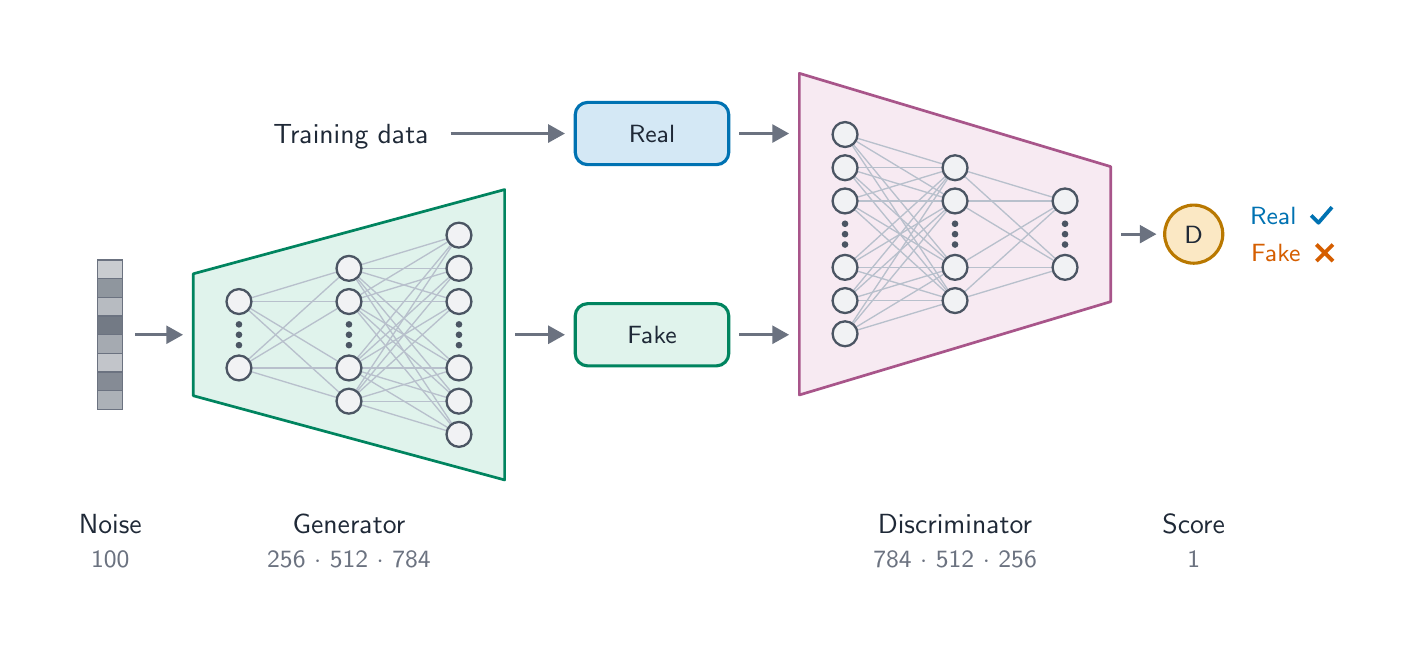
\begin{tikzpicture}[x=0.75pt, y=-0.75pt]
  \tikzset{
    xm funnel 18a79of/.style={fill=xm2, draw=xm3, line width=0.98pt, line join=round},
    xm funnel 1dcnepv/.style={fill=xm4, draw=xm5, line width=0.98pt, line join=round},
    xm arrow 1l69f7x/.style={draw=xm6, line width=1.05pt},
    xm arrow 19pejvw/.style={fill=xm6, line join=round},
    xm box 13pbqni/.style={fill=xm7, draw=xm6, line width=0.45pt},
    xm box 13w2a8d/.style={fill=xm8, draw=xm6, line width=0.45pt},
    xm box 142stt8/.style={fill=xm9, draw=xm6, line width=0.45pt},
    xm box 1unt8g8/.style={fill=xm10, draw=xm6, line width=0.45pt},
    xm box 1uujs13/.style={fill=xm11, draw=xm6, line width=0.45pt},
    xm box 1v1ably/.style={fill=xm12, draw=xm6, line width=0.45pt},
    xm box 1v80v6t/.style={fill=xm13, draw=xm6, line width=0.45pt},
    xm box 1verero/.style={fill=xm14, draw=xm6, line width=0.45pt},
    xm edge 170dxcz/.style={draw=xm15, line width=0.48pt},
    xm node hvhhxc/.style={fill=xm16, draw=xm17, line width=0.83pt},
    xm circle 1g24ir9/.style={fill=xm17},
    xm box 442wj7/.style={fill=xm18, draw=xm19, line width=1.13pt, rounded corners=4.5pt},
    xm box 4erm6b/.style={fill=xm2, draw=xm3, line width=1.13pt, rounded corners=4.5pt},
    xm node 1tdv5pi/.style={fill=xm20, draw=xm21, line width=1.13pt},
    xm mark moeldj/.style={draw=xm19, line width=1.35pt, line join=round},
    xm mark bi72rz/.style={draw=xm22, line width=1.35pt, line join=round},
    xm text xm23/.style={text=xm23, inner sep=0},
    xm text xm19/.style={text=xm19, inner sep=0},
    xm text xm22/.style={text=xm22, inner sep=0},
    xm text xm6/.style={text=xm6, inner sep=0},
  }
  \fill[xm1] (0,0) rectangle (654.91,285.15);
  % Diagram
  \path[xm funnel 18a79of] (79.8,118.57) -- (229.8,78) -- (229.8,217.9) -- (79.8,177.33) -- cycle;
  \path[xm funnel 1dcnepv] (371.8,22) -- (521.8,66.94) -- (521.8,132.01) -- (371.8,176.95) -- cycle;
  \path[xm arrow 1l69f7x] (51.8,147.95) -- (67.8,147.95);
  \path[xm arrow 19pejvw] (74.8,147.95) -- (66.8,152.45) -- (66.8,143.45) -- cycle;
  \path[xm arrow 1l69f7x] (234.8,147.95) -- (251.8,147.95);
  \path[xm arrow 19pejvw] (258.8,147.95) -- (250.8,152.45) -- (250.8,143.45) -- cycle;
  \path[xm arrow 1l69f7x] (342.8,147.95) -- (359.8,147.95);
  \path[xm arrow 19pejvw] (366.8,147.95) -- (358.8,152.45) -- (358.8,143.45) -- cycle;
  \path[xm arrow 1l69f7x] (342.8,51) -- (359.8,51);
  \path[xm arrow 19pejvw] (366.8,51) -- (358.8,55.5) -- (358.8,46.5) -- cycle;
  \path[xm arrow 1l69f7x] (203.8,51) -- (251.8,51);
  \path[xm arrow 19pejvw] (258.8,51) -- (250.8,55.5) -- (250.8,46.5) -- cycle;
  \path[xm arrow 1l69f7x] (526.8,99.48) -- (536.8,99.48);
  \path[xm arrow 19pejvw] (543.8,99.48) -- (535.8,103.98) -- (535.8,94.98) -- cycle;
  \path[xm box 13pbqni] (33.8,111.95) rectangle ++(12,9);
  \path[xm box 13w2a8d] (33.8,120.95) rectangle ++(12,9);
  \path[xm box 142stt8] (33.8,129.95) rectangle ++(12,9);
  \path[xm box 1unt8g8] (33.8,138.95) rectangle ++(12,9);
  \path[xm box 1uujs13] (33.8,147.95) rectangle ++(12,9);
  \path[xm box 1v1ably] (33.8,156.95) rectangle ++(12,9);
  \path[xm box 1v80v6t] (33.8,165.95) rectangle ++(12,9);
  \path[xm box 1verero] (33.8,174.95) rectangle ++(12,9);
  \path[xm edge 170dxcz] (107.54,130.22) -- (149.05,117.68);
  \path[xm edge 170dxcz] (107.8,131.95) -- (148.8,131.95);
  \path[xm edge 170dxcz] (106.94,135.05) -- (149.66,160.85);
  \path[xm edge 170dxcz] (106.25,135.98) -- (150.35,175.92);
  \path[xm edge 170dxcz] (106.25,159.92) -- (150.35,119.98);
  \path[xm edge 170dxcz] (106.94,160.85) -- (149.66,135.05);
  \path[xm edge 170dxcz] (107.8,163.95) -- (148.8,163.95);
  \path[xm edge 170dxcz] (107.54,165.68) -- (149.05,178.22);
  \path[xm edge 170dxcz] (160.54,114.22) -- (202.05,101.68);
  \path[xm edge 170dxcz] (160.8,115.95) -- (201.8,115.95);
  \path[xm edge 170dxcz] (160.54,117.68) -- (202.05,130.22);
  \path[xm edge 170dxcz] (159.25,119.98) -- (203.35,159.92);
  \path[xm edge 170dxcz] (158.63,120.57) -- (203.97,175.33);
  \path[xm edge 170dxcz] (158.11,120.95) -- (204.49,190.95);
  \path[xm edge 170dxcz] (159.94,128.85) -- (202.66,103.05);
  \path[xm edge 170dxcz] (160.54,130.22) -- (202.05,117.68);
  \path[xm edge 170dxcz] (160.8,131.95) -- (201.8,131.95);
  \path[xm edge 170dxcz] (159.94,135.05) -- (202.66,160.85);
  \path[xm edge 170dxcz] (159.25,135.98) -- (203.35,175.92);
  \path[xm edge 170dxcz] (158.63,136.57) -- (203.97,191.33);
  \path[xm edge 170dxcz] (158.63,159.33) -- (203.97,104.57);
  \path[xm edge 170dxcz] (159.25,159.92) -- (203.35,119.98);
  \path[xm edge 170dxcz] (159.94,160.85) -- (202.66,135.05);
  \path[xm edge 170dxcz] (160.8,163.95) -- (201.8,163.95);
  \path[xm edge 170dxcz] (160.54,165.68) -- (202.05,178.22);
  \path[xm edge 170dxcz] (159.94,167.05) -- (202.66,192.85);
  \path[xm edge 170dxcz] (158.11,174.95) -- (204.49,104.95);
  \path[xm edge 170dxcz] (158.63,175.33) -- (203.97,120.57);
  \path[xm edge 170dxcz] (159.25,175.92) -- (203.35,135.98);
  \path[xm edge 170dxcz] (160.54,178.22) -- (202.05,165.68);
  \path[xm edge 170dxcz] (160.8,179.95) -- (201.8,179.95);
  \path[xm edge 170dxcz] (160.54,181.68) -- (202.05,194.22);
  \path[xm node hvhhxc] (101.8,131.95) circle[radius=6];
  \path[xm circle 1g24ir9] (101.8,142.95) circle[radius=1.6];
  \path[xm circle 1g24ir9] (101.8,147.95) circle[radius=1.6];
  \path[xm circle 1g24ir9] (101.8,152.95) circle[radius=1.6];
  \path[xm node hvhhxc] (101.8,163.95) circle[radius=6];
  \path[xm node hvhhxc] (154.8,115.95) circle[radius=6];
  \path[xm node hvhhxc] (154.8,131.95) circle[radius=6];
  \path[xm circle 1g24ir9] (154.8,142.95) circle[radius=1.6];
  \path[xm circle 1g24ir9] (154.8,147.95) circle[radius=1.6];
  \path[xm circle 1g24ir9] (154.8,152.95) circle[radius=1.6];
  \path[xm node hvhhxc] (154.8,163.95) circle[radius=6];
  \path[xm node hvhhxc] (154.8,179.95) circle[radius=6];
  \path[xm node hvhhxc] (207.8,99.95) circle[radius=6];
  \path[xm node hvhhxc] (207.8,115.95) circle[radius=6];
  \path[xm node hvhhxc] (207.8,131.95) circle[radius=6];
  \path[xm circle 1g24ir9] (207.8,142.95) circle[radius=1.6];
  \path[xm circle 1g24ir9] (207.8,147.95) circle[radius=1.6];
  \path[xm circle 1g24ir9] (207.8,152.95) circle[radius=1.6];
  \path[xm node hvhhxc] (207.8,163.95) circle[radius=6];
  \path[xm node hvhhxc] (207.8,179.95) circle[radius=6];
  \path[xm node hvhhxc] (207.8,195.95) circle[radius=6];
  \path[xm box 442wj7] (263.8,36) rectangle ++(74,30);
  \path[xm box 4erm6b] (263.8,132.95) rectangle ++(74,30);
  \path[xm edge 170dxcz] (399.54,53.21) -- (441.05,65.74);
  \path[xm edge 170dxcz] (398.94,54.58) -- (441.66,80.37);
  \path[xm edge 170dxcz] (397.63,56.1) -- (442.97,110.85);
  \path[xm edge 170dxcz] (397.11,56.48) -- (443.49,126.47);
  \path[xm edge 170dxcz] (399.8,67.48) -- (440.8,67.48);
  \path[xm edge 170dxcz] (399.54,69.21) -- (441.05,81.74);
  \path[xm edge 170dxcz] (398.25,71.5) -- (442.35,111.45);
  \path[xm edge 170dxcz] (397.63,72.1) -- (442.97,126.85);
  \path[xm edge 170dxcz] (399.54,81.74) -- (441.05,69.21);
  \path[xm edge 170dxcz] (399.8,83.48) -- (440.8,83.48);
  \path[xm edge 170dxcz] (398.94,86.58) -- (441.66,112.37);
  \path[xm edge 170dxcz] (398.25,87.5) -- (442.35,127.45);
  \path[xm edge 170dxcz] (398.25,111.45) -- (442.35,71.5);
  \path[xm edge 170dxcz] (398.94,112.37) -- (441.66,86.58);
  \path[xm edge 170dxcz] (399.8,115.48) -- (440.8,115.48);
  \path[xm edge 170dxcz] (399.54,117.21) -- (441.05,129.74);
  \path[xm edge 170dxcz] (397.63,126.85) -- (442.97,72.1);
  \path[xm edge 170dxcz] (398.25,127.45) -- (442.35,87.5);
  \path[xm edge 170dxcz] (399.54,129.74) -- (441.05,117.21);
  \path[xm edge 170dxcz] (399.8,131.48) -- (440.8,131.48);
  \path[xm edge 170dxcz] (397.11,142.47) -- (443.49,72.48);
  \path[xm edge 170dxcz] (397.63,142.85) -- (442.97,88.1);
  \path[xm edge 170dxcz] (398.94,144.37) -- (441.66,118.58);
  \path[xm edge 170dxcz] (399.54,145.74) -- (441.05,133.21);
  \path[xm edge 170dxcz] (452.54,69.21) -- (494.05,81.74);
  \path[xm edge 170dxcz] (451.25,71.5) -- (495.35,111.45);
  \path[xm edge 170dxcz] (452.8,83.48) -- (493.8,83.48);
  \path[xm edge 170dxcz] (451.94,86.58) -- (494.66,112.37);
  \path[xm edge 170dxcz] (451.94,112.37) -- (494.66,86.58);
  \path[xm edge 170dxcz] (452.8,115.48) -- (493.8,115.48);
  \path[xm edge 170dxcz] (451.25,127.45) -- (495.35,87.5);
  \path[xm edge 170dxcz] (452.54,129.74) -- (494.05,117.21);
  \path[xm node hvhhxc] (393.8,51.48) circle[radius=6];
  \path[xm node hvhhxc] (393.8,67.48) circle[radius=6];
  \path[xm node hvhhxc] (393.8,83.48) circle[radius=6];
  \path[xm circle 1g24ir9] (393.8,94.48) circle[radius=1.6];
  \path[xm circle 1g24ir9] (393.8,99.48) circle[radius=1.6];
  \path[xm circle 1g24ir9] (393.8,104.48) circle[radius=1.6];
  \path[xm node hvhhxc] (393.8,115.48) circle[radius=6];
  \path[xm node hvhhxc] (393.8,131.48) circle[radius=6];
  \path[xm node hvhhxc] (393.8,147.48) circle[radius=6];
  \path[xm node hvhhxc] (446.8,67.48) circle[radius=6];
  \path[xm node hvhhxc] (446.8,83.48) circle[radius=6];
  \path[xm circle 1g24ir9] (446.8,94.48) circle[radius=1.6];
  \path[xm circle 1g24ir9] (446.8,99.48) circle[radius=1.6];
  \path[xm circle 1g24ir9] (446.8,104.48) circle[radius=1.6];
  \path[xm node hvhhxc] (446.8,115.48) circle[radius=6];
  \path[xm node hvhhxc] (446.8,131.48) circle[radius=6];
  \path[xm node hvhhxc] (499.8,83.48) circle[radius=6];
  \path[xm circle 1g24ir9] (499.8,94.48) circle[radius=1.6];
  \path[xm circle 1g24ir9] (499.8,99.48) circle[radius=1.6];
  \path[xm circle 1g24ir9] (499.8,104.48) circle[radius=1.6];
  \path[xm node hvhhxc] (499.8,115.48) circle[radius=6];
  \path[xm node 1tdv5pi] (561.8,99.48) circle[radius=14];
  \path[xm mark moeldj] (618.41,90.48) -- (621.91,93.98) -- (628.41,86.48);
  \path[xm mark bi72rz] (620.91,104.48) -- (628.91,112.48) (628.91,104.48) -- (620.91,112.48);
  \node[xm text xm23, font=\sffamily\fontsize{9}{10.8}\selectfont, anchor=base] at (300.8,55.37) {Real};
  \node[xm text xm23, font=\sffamily\fontsize{9}{10.8}\selectfont, anchor=base] at (300.8,152.32) {Fake};
  \node[xm text xm23, font=\sffamily\fontsize{9.75}{11.7}\selectfont, anchor=base] at (155.79,55.73) {Training data};
  \node[xm text xm23, font=\sffamily\fontsize{9}{10.8}\selectfont, anchor=base] at (561.8,103.84) {D};
  \node[xm text xm19, font=\sffamily\fontsize{9}{10.8}\selectfont, anchor=base] at (600.11,94.84) {Real};
  \node[xm text xm22, font=\sffamily\fontsize{9}{10.8}\selectfont, anchor=base] at (601.35,112.84) {Fake};
  \node[xm text xm23, font=\sffamily\fontsize{9.75}{11.7}\selectfont, anchor=base] at (39.8,243.49) {Noise};
  \node[xm text xm6, font=\sffamily\fontsize{9}{10.8}\selectfont, anchor=base] at (39.8,260.26) {100};
  \node[xm text xm23, font=\sffamily\fontsize{9.75}{11.7}\selectfont, anchor=base] at (154.8,243.49) {Generator};
  \node[xm text xm6, font=\sffamily\fontsize{9}{10.8}\selectfont, anchor=base] at (154.8,260.26) {256 \ensuremath{\cdot} 512 \ensuremath{\cdot} 784};
  \node[xm text xm23, font=\sffamily\fontsize{9.75}{11.7}\selectfont, anchor=base] at (446.8,243.49) {Discriminator};
  \node[xm text xm6, font=\sffamily\fontsize{9}{10.8}\selectfont, anchor=base] at (446.8,260.26) {784 \ensuremath{\cdot} 512 \ensuremath{\cdot} 256};
  \node[xm text xm23, font=\sffamily\fontsize{9.75}{11.7}\selectfont, anchor=base] at (561.8,243.49) {Score};
  \node[xm text xm6, font=\sffamily\fontsize{9}{10.8}\selectfont, anchor=base] at (561.8,260.26) {1};
\end{tikzpicture}
\end{document}
